\documentclass[a4paper,11pt]{article}
\usepackage[utf8]{inputenc}
\usepackage[german]{babel}
\usepackage{geometry}
\usepackage{graphicx}
\usepackage{parskip}
\usepackage{titlesec}
\usepackage{hyperref}

\setcounter{secnumdepth}{4}

\titleformat{\paragraph}
{\normalfont\normalsize\bfseries}{\theparagraph}{1em}{}
\titlespacing*{\paragraph}
{0pt}{3.25ex plus 1ex minus .2ex}{1.5ex plus .2ex}

\geometry{a4paper, margin=2.5cm}
\graphicspath{{images/}}

\begin{document}

\begin{table}[h]
	\centering
	\footnotesize
	\begin{tabular}{| p{1.5cm} | p{2.5cm} | p{2cm} | p{2cm} | p{2cm} |}
		\hline
		                            & Verantwortliche Teammitglieder (Organisation, Anlegen der Dokumentenversion, Moderation, Abgabe)         & Anwesende während der Meetings                                                                           & (Online-) Beiträge zum Inhalt durch                                                                      & Korrektur-gelesen durch                                                                                  \\
		\hline
		Dokument Sprint 2 Version 1 & Paul Schröder, Eric Buthmann, Yanik Buthmann, Mathis Behrendt, Adrian Gode, Niklas Krüger, Kevin Zellmer & Paul Schröder, Eric Buthmann, Yanik Buthmann, Mathis Behrendt, Adrian Gode, Niklas Krüger, Kevin Zellmer & Paul Schröder, Eric Buthmann, Yanik Buthmann, Mathis Behrendt, Adrian Gode, Niklas Krüger, Kevin Zellmer & Paul Schröder, Eric Buthmann, Yanik Buthmann, Mathis Behrendt, Adrian Gode, Niklas Krüger, Kevin Zellmer \\
		\hline
	\end{tabular}
\end{table}

\section{Backlogs und Planung}

\subsection{Produktbacklog vor und nach dem Sprint}
Das Produktbacklog hat sich im Vergleich zum letzten Sprint nicht verändert.\\

\subsection{Sprint Planung}

Im letzten Sprint wurden folgende  User Stories vollständig umgesetzt: S1.1, S1.2, S5.1.
Das Resultat des letzten Sprints war ein Prototyp mit den genannten Features.\\
Es wurden nicht alle geplanten User Stories umgesetzt.
Diese wurden daher in den zweiten Sprint verschoben.
Namentlich sind das die User Stories S1.3, S4.1, S6.1.\\

\noindent\textit{Hinweis: Das vollständige Sprintbacklog ist unter \href{run:./Sprintbacklog.pdf}{Sprintbacklog.pdf}, sowie \href{https://git.informatik.uni-rostock.de/softwaretechnik-ws-2025-26/uebung3/team3/projekt-team3-uebung3/-/blob/main/abgabedokumente/Sprintbacklog.pdf?ref_type=heads}{im Gitlab} zu finden.}

\section{Verfeinerte Architektur}
\subsection{Task/User Stories}
\subsubsection{Modellierung für User Story S4.1: Backlogs erstellen}
\paragraph{Modellierung verfeinerter Struktur}

Im letzten Sprint wurde bereits an der Modellierung der User Story S4.1 gearbeitet.
Der Entwurf wurde geringfügig überarbeitet.
Das Klassendiagramm zu sehen in Abbildung \ref{fig:klassendiagramm_s4_1} zeigt die zu implementierenden Klassen für diese User Story.\\
Im Presentation Layer wird das Interface \textbf{IBacklogController} und die implementierende Klasse \textbf{BacklogController} hinzugefügt.
In dieser Klasse werden die Anfragen an die Route \textbf{GET /create-backlog} \textbf{POST /create-backlog} behandelt.\\
Im Service Layer wird das Interface \textbf{IBacklogService} und die implementierende Klasse \textbf{BacklogService} hinzugefügt.
Dort wird die Logik zum Erstellen eines Backlog implementiert.\\
Abschließend wird im Data Layer das Interface \textbf{IBacklogRepository} und die implementierende Klasse \textbf{BacklogRepository} hinzugefügt.
Hier wird die Logik zum Speichern eines Backlogs implementiert.

\begin{figure}[h]
	\centering
	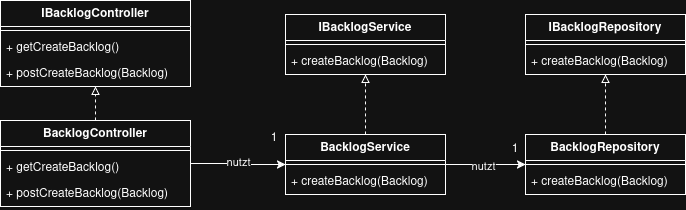
\includegraphics[width=10cm]{s4_1_klassendiagramm.png}
	\caption{Klassendiagramm für User Story S4.1}
	\label{fig:klassendiagramm_s4_1}
\end{figure}


\paragraph{Modellierung verfeinerter Interfaces und Datenstrukturen}

Für das Anlegen eines Backlogs wird die Datenstruktur \textbf{Backlog} benötigt.
Die Abbildung \ref{fig:klassendiagramm_datenstrukturen_s4_1} zeigt die zu implementierende Klasse und ihre Beziehung zu der Klasse \textbf{Task}.
Der Entwurf dieser Datenstruktur ist nicht final und wird bei der Umsetzung von weiteren User Stories angepasst.
Für die Umsetzung dieser User Story ist dieser Entwurf jedoch hinreichend.

\begin{figure}
	\centering
	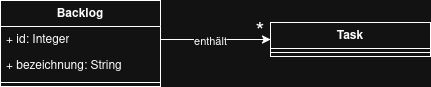
\includegraphics[width=10cm]{s4_1_datenstrukturen.png}
	\caption{Klassendiagramm der Datenstrukturen für User Story S4.1}
	\label{fig:klassendiagramm_datenstrukturen_s4_1}
\end{figure}


\paragraph{Modellierung relevanter Verhaltensaspekte}
Beim Anlegen eines Backlogs muss beachten werden, dass ein Backlog mit der gleichen Bezeichnung bereits existieren kann.
Wie in Abbildung \ref{fig:sequenzdiagramm_s4_1} zu sehen, muss in diesem Fall die Klasse \textbf{BacklogRepository} die Situation erkennen und eine Fehlermeldung an die darüber liegenden Schichten weiterleiten.
Die Klasse \textbf{BacklogController} muss darauf die Anzeige der Fehlermeldung einleiten.
Andernfalls werden in der Klasse \textbf{BacklogRepository} die Daten des Backlogs in der Datenbank gespeichert.

\begin{figure}
	\centering
	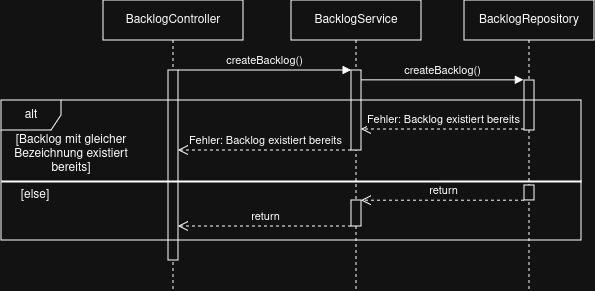
\includegraphics[width=10cm]{s4_1_sequenzdiagramm.png}
	\caption{Sequenzdiagramm für User Story S4.1}
	\label{fig:sequenzdiagramm_s4_1}
\end{figure}


\subsection{Tracing}

\section{Implementation und Tests}
\subsection{Updates zu den genutzen Technologien}
\subsection{Dokumentation der Codequalität}

\end{document}





